\documentclass[a4paper]{article}

%% Language and font encodings
\usepackage[english]{babel}
\usepackage[utf8x]{inputenc}

\usepackage{booktabs}
\usepackage{tabu}
\usepackage[T1]{fontenc}

%% Sets page size and margins
\usepackage[a4paper,top=3cm,bottom=2cm,left=3cm,right=3cm,marginparwidth=1.75cm]{geometry}

%% Useful packages
\usepackage{amsmath}
\usepackage{graphicx}
\usepackage{titling}
%\usepackage{apacite}
\usepackage[colorinlistoftodos]{todonotes}
\usepackage[colorlinks=true, allcolors=blue]{hyperref}
\usepackage[strings]{underscore}


\title{Modeling and 3D Printing Sea Shells\\
		\large Final Report}
\author{Edward Ye || 100972832}
\date{2019-04-15}

\begin{document}
\maketitle

\begin{abstract}
	I thought sea shells were cool so I made some models and 3D printed them.
\end{abstract}

\section*{Some Background and Motivation}

Sea shells have interesting patterns which  appear to be readily described by mathematics and computation. Work has already been done to describe aspects of sea shells, from the spiral shape to the color patterns to the protrusions found on the exterior \cite{Galbraith00modelingmurex}\cite{abss}\cite{VANDERHELM1998505}. Recently some work has also gone into the 3D printing of sea shell model \cite{3dprinting-seashells}\cite{bachman-3dprinting}.

The motivation of this project will be to extend the methods of generating the exterior protrusions to be able to mimic a wider variety of shells. Prusinkiewicz and Fowler have modeled periodic ridge and bump patterns and they have also combined multiple generating curves to imitate more intricate shells \cite{abss}. Galbraith et al. have used constructive solid geometry (CSG) to compose different modules to generate a complete Murex Cabritii model. They have proposed the use of reaction-diffusion (RD) to place protrusions algorithmically \cite{Galbraith00modelingmurex}. Intuitively this appears to be a reasonable idea since the protrusion placement of certain shells are something like the placement of spots upon a leopard. Such patterns have already been described as textures using RD \cite{Turk:1991:GTA:127719.122749}.

\section*{Main Objective}

An interesting candidate for such a method would be:

\begin{figure}[h]
	\centering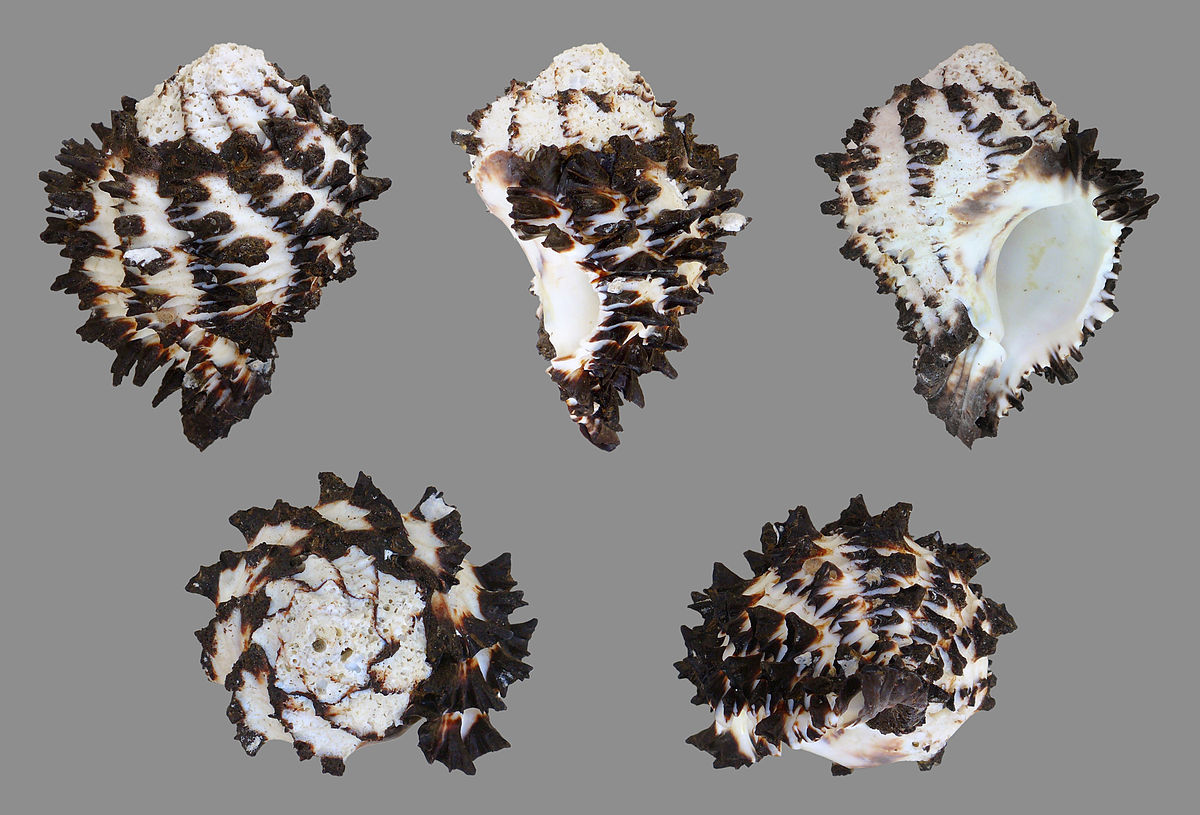
\includegraphics[scale=0.25]{./img/hexaplex_radix.jpg}
	\caption{Hexaplex radix \cite{wikipedia-hexaplex}}
	\label{fig:hexaplex-radix} % Unique label used for referencing the figure in-text
	%\addcontentsline{toc}{figure}{Figure \ref{fig:placeholder}} % Uncomment to add the figure to the table of contents
\end{figure}

The main objective would be to create a model that closely resembles the shell and to 3D print it. After completing the main objective it may be possible to generalize the methods used to describe various other shells.

\bibliographystyle{plain}
\bibliography{refs}

\end{document}